%%%%%%%%%%%%%%%%%%%%%%%%%%%%%%%%%%%%%%%%%%%%%%%%%%%%%%%%%%%%%%%%%%%%%%%%
% Plantilla TFG/TFM
% Universidad de A Coruña. Facultad de Informática
% Realizado por: Welton Vieira dos Santos
% Modificado: Welton Vieira dos Santos
% Contacto: welton.dossantos@udc.es
%%%%%%%%%%%%%%%%%%%%%%%%%%%%%%%%%%%%%%%%%%%%%%%%%%%%%%%%%%%%%%%%%%%%%%%%


\chapter{Modelo de conocimiento}
\newpage
\section{Fase de identificación}
\subsection{Tareas del formulario OM-3}
La tarea elegida para este modelo conceptual ha sido la tarea 5 del OM-3 (Tabla \ref{tab:IdentificacionOM3}), que corresponde con la \textbf{Gestión de las Operativas Abiertas}.

\begin{table}[H]
  \centering
  \resizebox{18,0cm}{!}{
    \begin{tabular}{|c|c|c|c|c|c|c|}
      \hline
      \multicolumn{3}{|c}{\textbf{Modelo de Organización}} & \multicolumn{4}{|c|}{\textbf{Formulario OM-3: Descomposición de los Procesos}}\\
      \hline \hline
      \textsc{N\textordmasculine} & \textsc{Tarea} & \textsc{Realiza\-da por} & \textsc{¿Dónde?} & \textsc{Recursos de Conocimiento} & \textsc {¿In\-ten\-si\-va en Conocimiento?} & \textsc{Im\-por\-tan\-cia} \\
      \hline
            
      5 & \multicolumn{1}{|p{6.0cm}|}{\centering Gestionar las operativas abiertas} & \multicolumn{1}{|p{6.0cm}|}{\centering Inversor (usuario)} &  \multicolumn{1}{|p{5.0cm}|}{\centering En PC del inversor (usuario)} & \multicolumn{1}{|p{6.0cm}|}{\centering Experiencia en gestionar las operativas de compra y venta de activos al mercado de divisas. Teorías de gestión de capital de inversión} & Sí (elevado) & Máxima \\
      \hline
    \end{tabular}
  }
	\caption{\label{tab:IdentificacionOM3}Tarea elegida para el modelo de conocimiento}
\end{table}

\subsection{Glosario de términos}
\begin{itemize}
	\item \textbf{Activo:} Entidad en la que se prentende especular, que en caso de Forex, hay una variabilidad de 26 pares de divisas, por ejemplo, EURUSD - Euro contra el Dolar.
	\item \textbf{Tendencia Alcista:} es una tendencia del mercado bulsátil donde los precios de los activos financieros llegan a nuevos máximos comparando en un mismo período de análisis. Ejemplo en la imagen de la izquierda de la Figura \ref{fig:EjemploTentendias}.
	\item \textbf{Tendencia Bajista:} es una tendencia del mercado bulsátil donde los precios de los activos financieros llegan a nuevos mínimos comparando en un mismo período de análisis. Ejemplo en la imagen de la derecha de la Figura \ref{fig:EjemploTentendias}.
	\item \textbf{Soporte:} Un soporte es un nivel de precio por debajo del actual, se espera que la fuerza de compra supere a la de venta, por lo que un impulso bajista se verá frenado y por lo tanto el precio repuntará. Normalmente, un soporte corresponde a un mínimo alcanzado anteriormente. Ejemplos en la Figura \ref{fig:SoportesResistencias} se muestra como lineas horizontales de color azul (S1,S2,\dots,SN)
	\item \textbf{Resistencia:} Una resistencia es el concepto opuesto a un soporte. Es un precio por encima del actual, la fuerza de venta superará a la de compra, poniendo fin al impulso alcista, y por lo tanto el precio retrocederá. Ejemplos en la Figura \ref{fig:SoportesResistencias} se muestra como lineas horizontales de color azul (S1,S2,\dots,SN).
	\item \textbf{Stop Loss:} Son límites máximos de pérdida puesto por parte del inversor para frenar una situación de pérdida.
\end{itemize}

\begin{figure}[H]
	\centering
	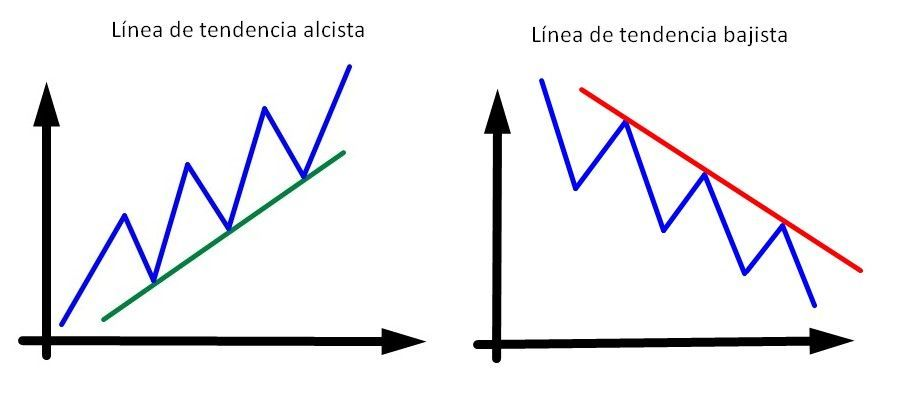
\includegraphics[scale=0.45]{imagenes/EjemploTentendias.png}
	\caption{\label{fig:EjemploTentendias}Ejemplo de tendencias de mercado}
\end{figure}

\begin{figure}[H]
	\centering
	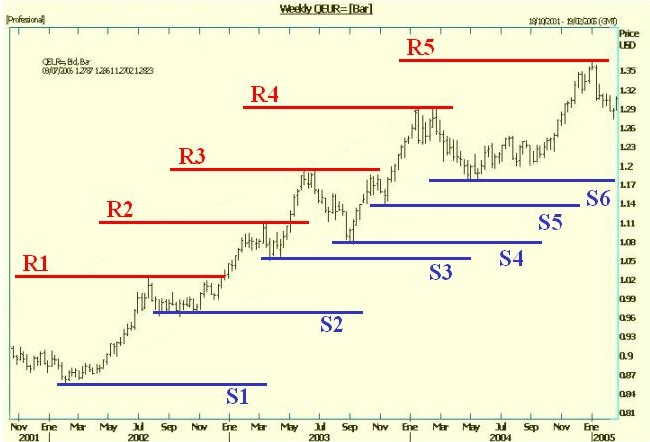
\includegraphics[scale=0.45]{imagenes/SoportesResistencias.png}
	\caption{\label{fig:SoportesResistencias}Soportes y resistencias del Euro/Dólar de 2001 a 2005}
\end{figure}

\subsection{Descripción de escenarios}
\begin{enumerate}
	\item  \textbf{Escenario de reducción de riesgo de una orden de compra (Buy):} En la situación que se muestra en la Figura \ref{fig:Situacion1}, donde el inversor había ejecutado una orden de compra en el precio \textbf{1.18767} y ha estipulado su gestión de riesgo para el precio \textbf{1.18664} y como se observa en el gráfico de la figura comentada anteriormente, el precio esta a favor del inversor y en esa ocasión el inversor tiene que reducir el riesgo inicial de la inversión al precio \textbf{1.19516} como se muestra en la Figura \ref{fig:Situacion12}.	
	\item  \textbf{Escenario de gestión de ganancia en una orden de compra (Buy)}: En la situación que se muestra en la Figura \ref{fig:Situacion2}, donde el inversor había ejecutado una orden de compra en el precio \textbf{1.18767} y ha estipulado su gestión de riesgo para el precio \textbf{1.18664} y como se observa en el gráfico de la figura comentada anteriormente, el precio esta a favor del inversor y el mismo decide cerrar esa operativa a precio del mercado, que en ese caso es de \textbf{1.19665}.	
\end{enumerate}
\begin{figure}[H]
    \centering
    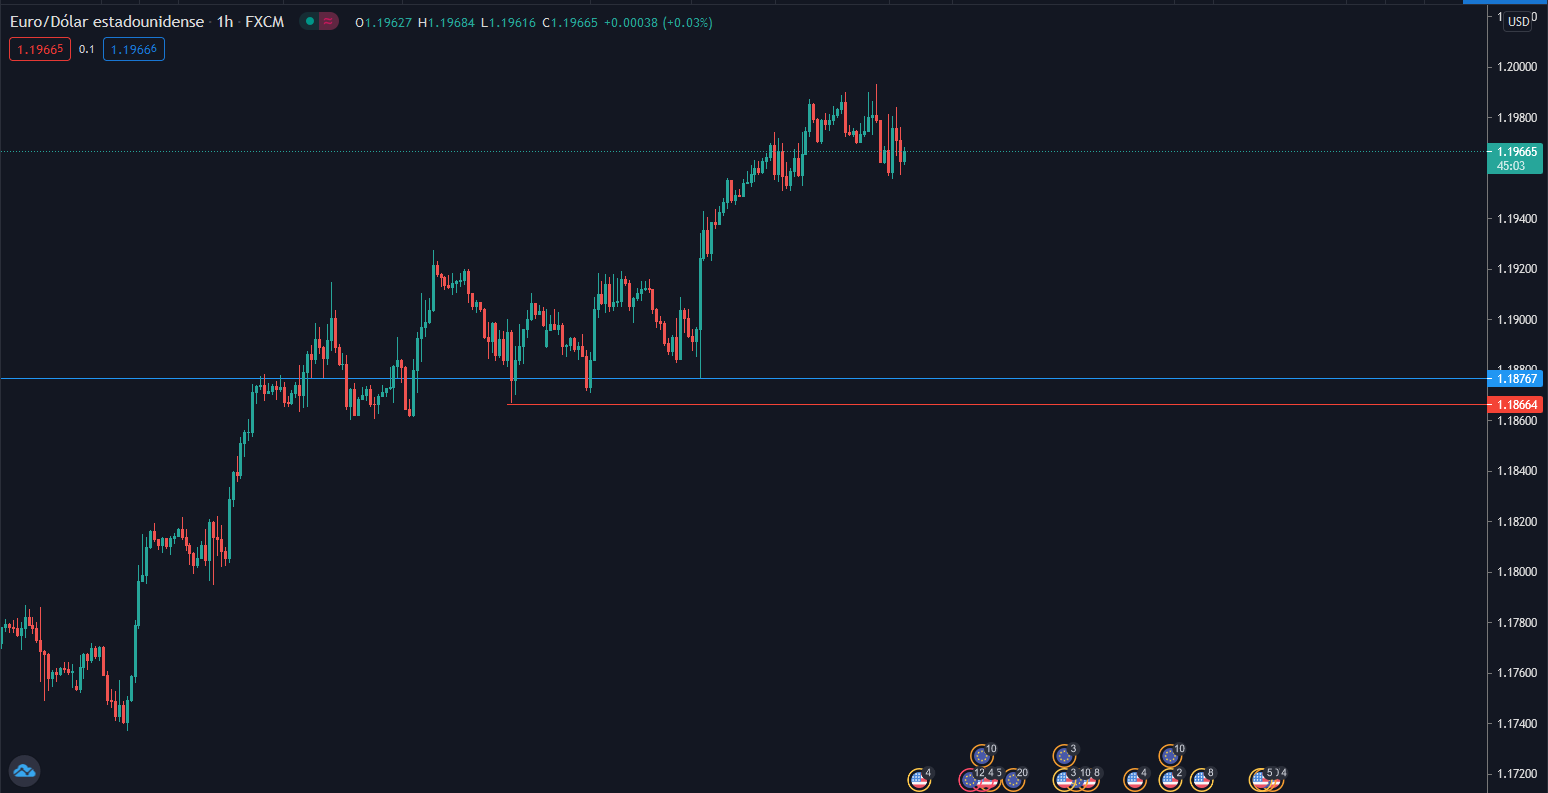
\includegraphics[scale=0.30]{imagenes/Situacion1.png}
    \caption{\label{fig:Situacion1}Ejemplo de una situación donde el inversor tiene que ajustar el riesgo de la operativa y seguir dentro del mercado}
  \end{figure}
\begin{figure}[H]
  \centering
  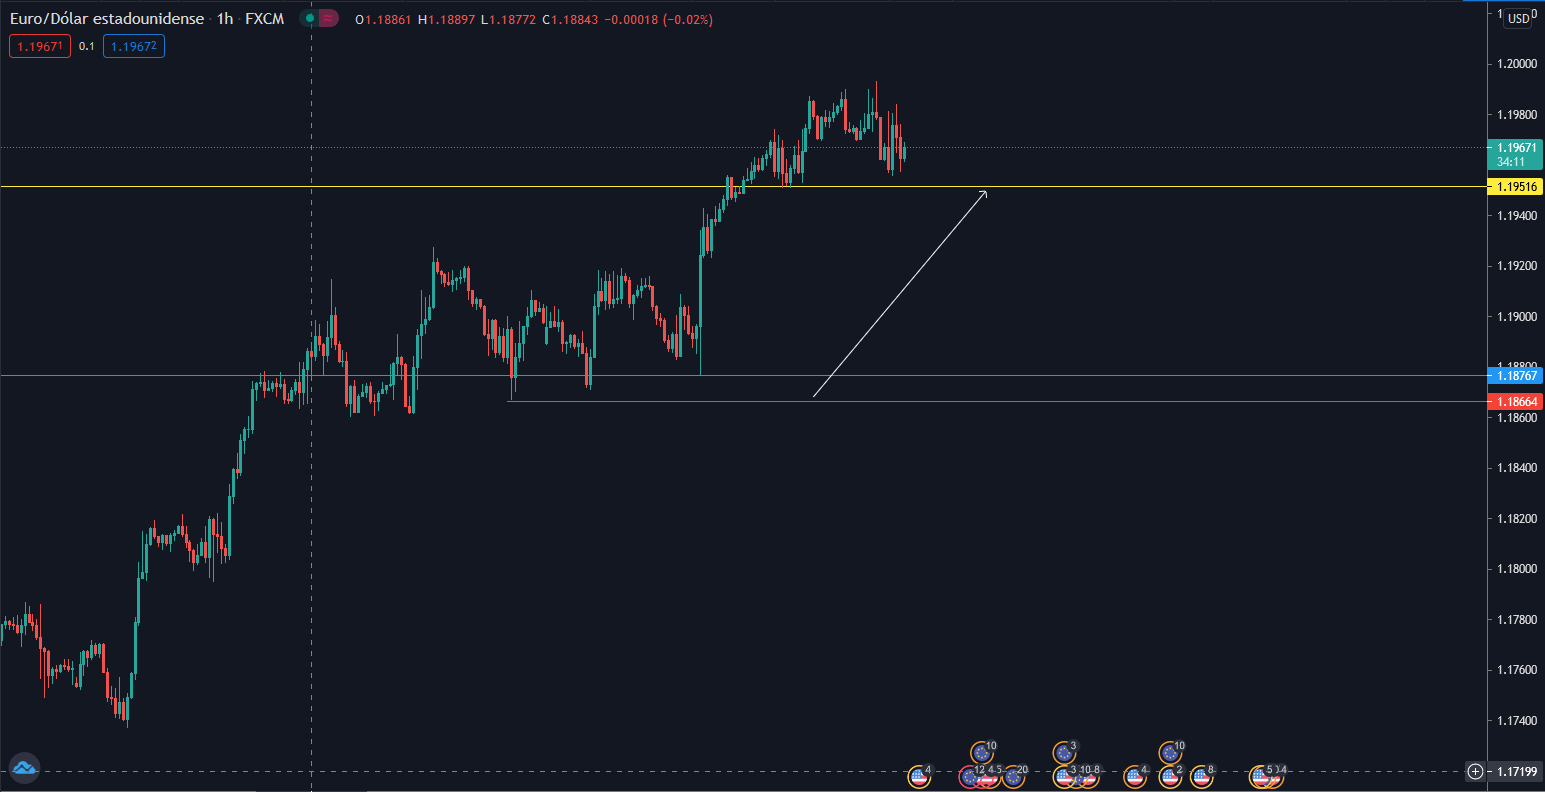
\includegraphics[scale=0.30]{imagenes/Situacion12.png}
  \caption{\label{fig:Situacion12}Ejemplo donde el inversor modifica el nivel de riesgo inicial y mantiene la orden de compra en el mercado}
\end{figure}
\begin{figure}[H]
  \centering
  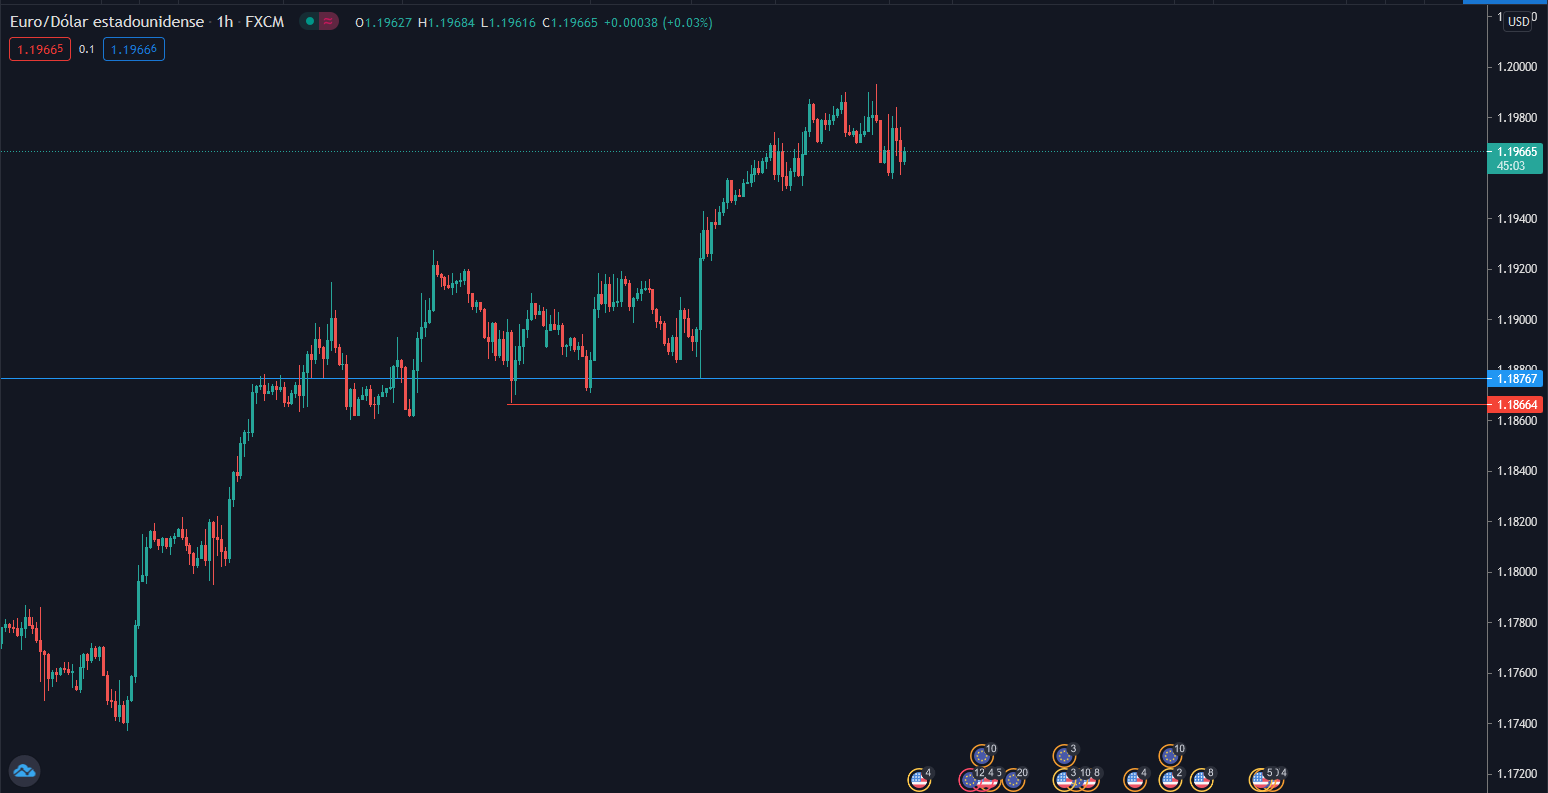
\includegraphics[scale=0.30]{imagenes/Situacion1.png}
  \caption{\label{fig:Situacion2}Ejemplo donde el inversor decide cerrar la orden de compra a precio de mercado}
\end{figure}

\section{Fase de especificación}
\subsection{Justificación de la selección de la metodología}
Para este proyecto hemos decidido utilizar la metodología ``middle-out'' con la selección de la plantilla de diagnóstico, ya que esa plantilla nos permite tomar varias decisiones un proyecto anterior con la misma metodología ``middle-out'', puesto que, además ser muy utilizada en nuestro caso sigue adaptandose perfectamente. 

\subsection{Plantilla anotada}

La plantilla que mas se adapta a nuestro problema es la de diagnóstico, como se muestra en la Figura \ref{fig:PlantillaEjemplo}. Con una pequeña modificación que se muestras en la Figuras \ref{fig:PlantillaDiagnosticoModificada}.

\begin{figure}[H]
  \centering
  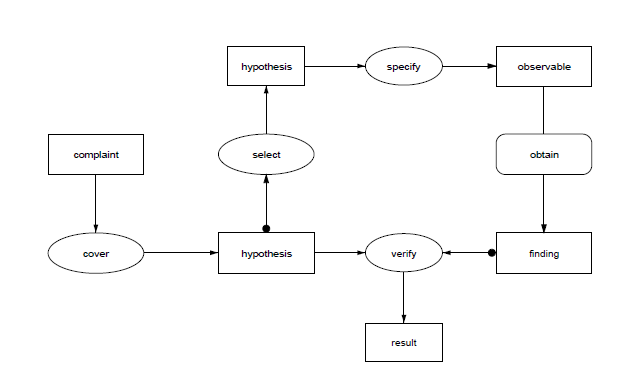
\includegraphics[scale=0.90]{imagenes/PlantillaEjemplo.png}
  \caption{\label{fig:PlantillaEjemplo}Ejemplo de la plantilla elegida}
\end{figure}

\begin{figure}[H]
  \centering
  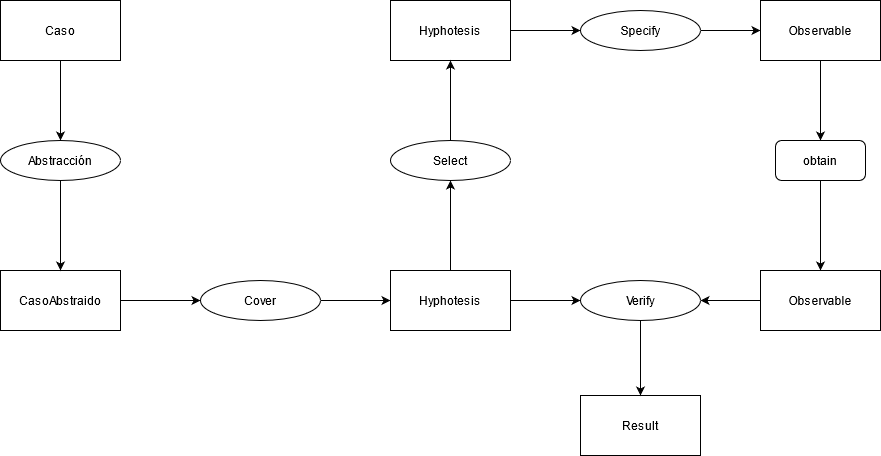
\includegraphics[scale=0.5]{imagenes/PlantillaDiagnosticoModificada.png}
  \caption{\label{fig:PlantillaDiagnosticoModificada}Ejemplo de la plantilla diagnóstico modificada}
\end{figure}

\subsubsection{Anotaciones}
Comentarios y ejemplos concretos para los roles presentes en la plantilla seleccionada.
\begin{itemize}
  \item \textbf{Caso:} Datos de una operativa: e.g. En la situación que se muestra en la Figura \ref{fig:Situacion1}, donde el inversor había ejecutado una orden de compra en el precio \textbf{1.18767} y ha estipulado su gestión de riesgo para el precio \textbf{1.18664} y como se observa en el gráfico de la figura comentada anteriormente, el precio esta a favor del inversor y en esa ocasión el inversor tiene que reducir el riesgo inicial de la inversión una vez superada la resistencia.
  \item \textbf{Caso abstraído:} Datos de una operativa abstaídos. e.g. El precio del activo ha superado la resistencia, es decir, MercadoForex.Activo.valor > resistencia. Se abstrae en MercadoForex.Activo.valor > MercadoForex.resistencia.Fuerte
  \item \textbf{Hypothesis\footnote{Hypothesis (Diferential)}:} Posibles acciones a llevar a cabo e.g. Cerrar la operativa, reducir el riesgo o No hacer nada.
  \item \textbf{Hypothesis\footnote{Hypothesis (Hypothesis)}:} Acción concreta a evaluar. e.g. reducir el riesgo.
  \item \textbf{Observable:} Estado del mercado de forex para la operativa actual. e.g. Mercado forex para EURUSD se mira la tendencia.
  \item \textbf{Finding:} Estado del mercado con respecto a nuestra operativa: e.g. Si estamos comprando que la tendencia sea alcista o si estamos vendiendo bajista.
  \item \textbf{Result:} Se confirma o deniega la hipotesis seleccionada. e.g. \{Ajustar riesgo = True, Cerrar la operativa = False\} 
\end{itemize}

\subsection{Esquema inicial del dominio}

\begin{figure}[H]
  \centering
  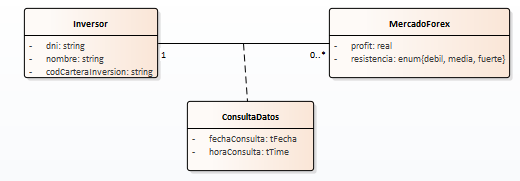
\includegraphics[scale=0.90]{imagenes/DominioInicial.png}
  \caption{\label{fig:DominioInicial}Dominio inicial}
\end{figure}

\subsection{Estructura inferencial}

\subsubsection{Plantilla}
\begin{figure}[H]
  \centering
  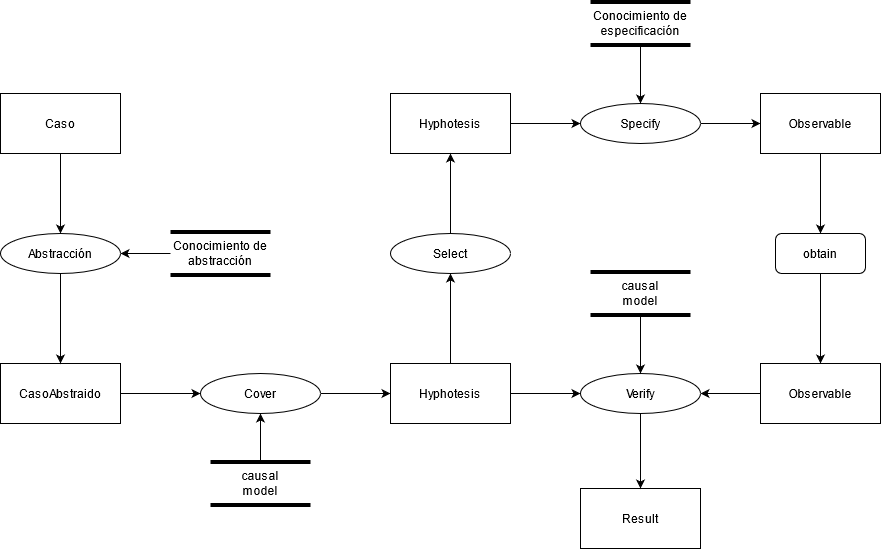
\includegraphics[scale=0.45]{imagenes/PlantillaDiagnosticoModificadaInferencia.png}
  \caption{\label{fig:PlantillaDiagnosticoModificadaInferencia}Plantilla diagnostico modificada con inferencias}
\end{figure}

\newpage

\subsubsection{Mapeado}
Relacción entre los roles de las inferencias de la plantilla con los conceptos de nuestro problema.

\begin{itemize}
  \item Abstraído:
  \begin{figure}[H]
    \centering
    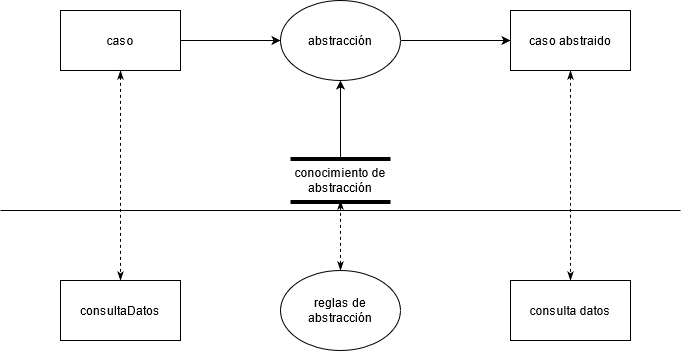
\includegraphics[scale=0.55]{imagenes/abstraccion_inferencia.png}
    \caption{\label{fig:Cover}Ejemplo del mapeo de Abstraccion}
  \end{figure}
  \item Cover:  
  \begin{figure}[H]
    \centering
    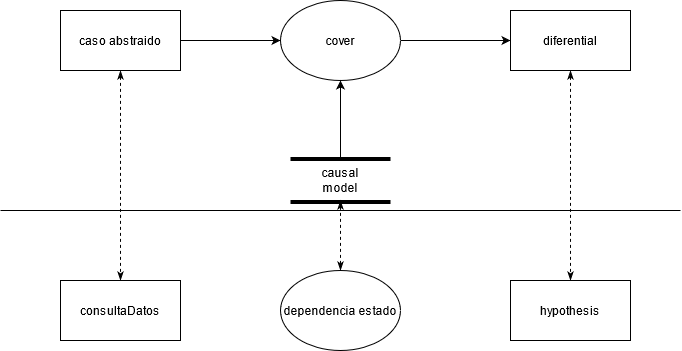
\includegraphics[scale=0.50]{imagenes/cover2.png}
    \caption{\label{fig:Cover}Ejemplo del mapeo de Cover}
  \end{figure}
  \item Select: 
  \begin{figure}[H]
    \centering
    \includegraphics[scale=0.50]{imagenes/select.png}
    \caption{\label{fig:Select}Ejemplo del mapeo de Select}
  \end{figure}
  \item Specify: 
  \begin{figure}[H]
    \centering
    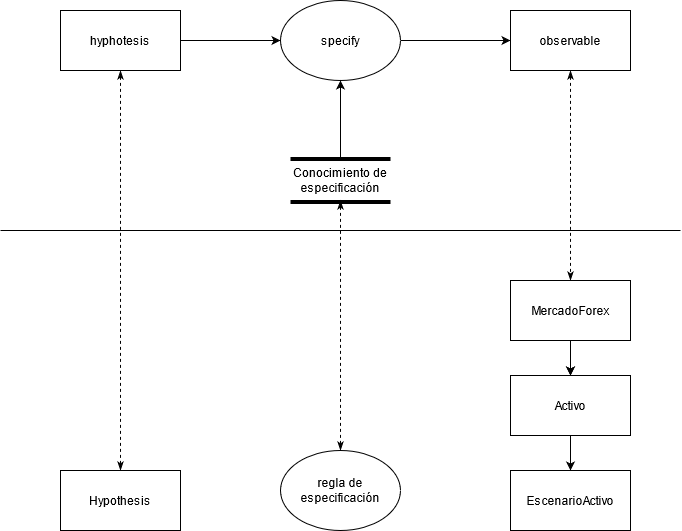
\includegraphics[scale=0.50]{imagenes/specify2.png}
    \caption{\label{fig:Specify}Ejemplo del mapeo de Specify}
  \end{figure}
  \item Obtain:  
  \begin{figure}[H]
    \centering
    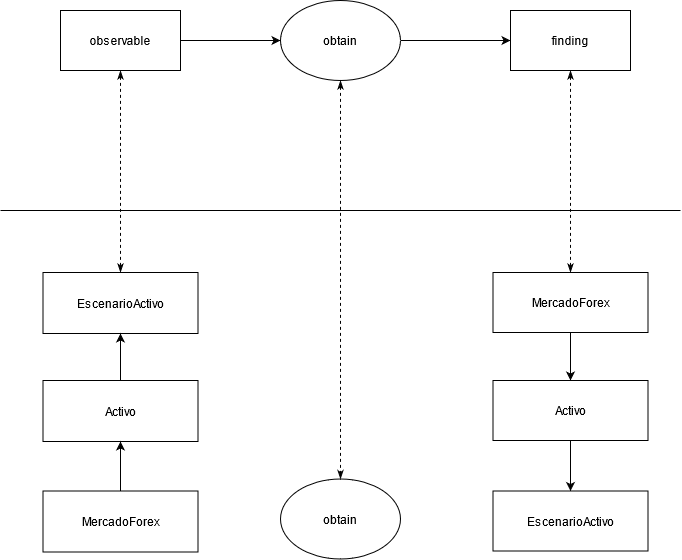
\includegraphics[scale=0.50]{imagenes/obtain2.png}
    \caption{\label{fig:Obtain}Ejemplo del mapeo de Obtain}
  \end{figure}
  \item Verify:  
  \begin{figure}[H]
    \centering
    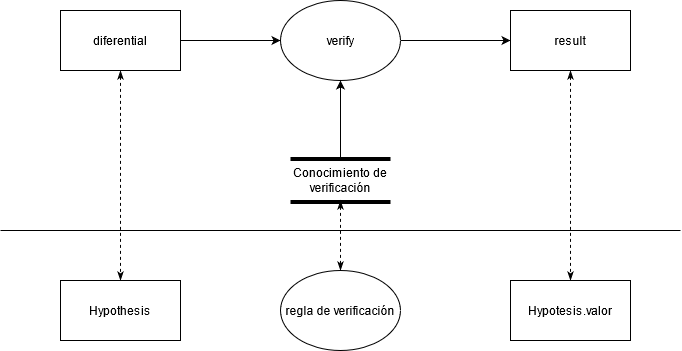
\includegraphics[scale=0.50]{imagenes/verify11.png}
    \caption{\label{fig:Verify}Ejemplo del mapeo de Verify del rol Diferential}
  \end{figure}
  \begin{figure}[H]
    \centering
    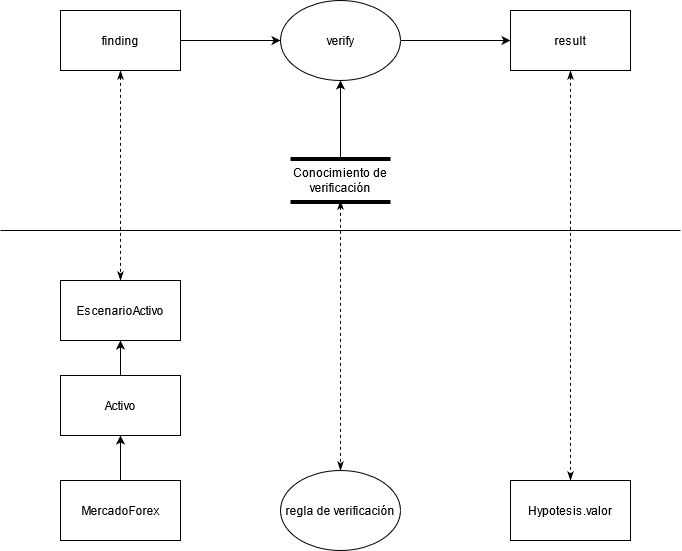
\includegraphics[scale=0.50]{imagenes/verify12.png}
    \caption{\label{fig:verify2}Ejemplo del mapeo de Verify del rol finding}
  \end{figure}
\end{itemize}

\section{Especificación y método de la tarea}

\subsection{Especificación}

\begin{lstlisting}[style=Python-color, caption={Pseudocódigo de la especificación}]
  TASK diagnosis;
  ROLES:
  INPUT: 
  caso abstraido: "Valor del activo y valor de la resistencia";
  OUTPUT:
  acción: "Posibles acciones a realizar(Cerraro operativa, reducir riesgo y no hacer nada) a causa del caso abstraído";
  Evidencia: "Resultados obtenidos durante el diagnostico";
  END TASK diagnosis;
\end{lstlisting}

\subsection{Método}

\begin{lstlisting}[style=Python-color, caption={Pseudocódigo de Completo}]  
  TASKMETHOD causalcovering;
  REALIZES: diagnosis;
    DECOMPOSITION:
    INFERENCES: cover, select, specify, verify;
    TRANSFER-FUNCTIONS: obtain;
    ROLES:
      INTERMEDIATE:
      differential: "active candidate solutions";
      hypothesis: "candidate solution";
      result: "boolean indicating result of the test";
      expected-finding: "data one would normally expect to find";
        actual-finding: "the data actually observed in practice";
        CONTROL-STRUCTURE:
        WHILE NEWSOLUTION cover(complaint -> hypothesis) DO
        differential := hypothesis ADD differential;
      END WHILE
      REPEAT
          select(differential -> hypothesis);
          specify(hypothesis -> observable);
          obtain(observable -> finding);
          evidence := finding ADD evidence;
          FOREACH hypothesis IN differential DO
          verify(hypothesis + evidence -> result);
          IF result == false
          THEN differential := differential SUBTRACT hypothesis;
          END IF
          END FOREACH
          UNTIL
        SIZE differential <= 1 OR "no more observables left";
        END REPEAT
    faults := differential;
    END TASKMETHOD causalcovering;
\end{lstlisting}


\subsection{Base de conocimiento}
\begin{lstlisting}[style=Python-color, caption={regla-abstraccion}]
  EXPRESSIONS:
    MercadoForex.Activo.EscenarioActivo.Resistencia.ultimoValor > max(MercadoForex.Activo.EscenarioActivo.Resistencia.historicoDatos) AND MercadoForex.Activo.EscenarioActivo.Resistencia.intentosRuptura > 3
  Abstraemos
    MercadoForex.Activo.EscenarioActivo.Resistencia.valorAbstraido = Fuerte
  END KNOWLEDGE-BASE dependencia-estado;
  
  EXPRESSIONS:
    MercadoForex.Activo.EscenarioActivo.Resistencia.ultimoValor > max(MercadoForex.Activo.EscenarioActivo.Resistencia.historicoDatos) AND MercadoForex.Activo.EscenarioActivo.Resistencia.intentosRuptura <= 3
  Abstraemos
    MercadoForex.Activo.EscenarioActivo.Resistencia.valorAbstraido = Debil
  END KNOWLEDGE-BASE dependencia-estado;
\end{lstlisting}

\begin{lstlisting}[style=Python-color, caption={dependencia-estado}]
  EXPRESSIONS:
    MercadoForex.Activo.valorActual > MercadoForex.Activo.EscenarioActivo.Resistencia.ultimoValor AND MercadoForex.Activo.EscenarioActivo.Resistencia.valorAbstraido = Fuerte
  CONDICIONA-A
    Hypothesis = {Ajustar_Riesgo, CerrarOperativa, NoHacerNada}
  END KNOWLEDGE-BASE dependencia-estado;
    
  EXPRESSIONS:
    MercadoForex.Activo.valorActual > MercadoForex.Activo.EscenarioActivo.Resistencia.ultimoValor
    AND MercadoForex.Activo.EscenarioActivo.Resistencia.valorAbstraido = Debil
  CONDICIONA-A
    Hypothesis = {CerrarOperativa, NoHacerNada}
  END KNOWLEDGE-BASE dependencia-estado;
\end{lstlisting}
    
\begin{lstlisting}[style=Python-color, caption={regla-especificación}]
  EXPRESSIONS:
    accion = AjustarRiesgo AND MercadoForex.Activo.tipo = compra
    RESULTA-EN
         MercadoForex.Activo.EscenarioActivo.Tendencia = alcista

  EXPRESSIONS:
    accion = AjustarRiesgo AND MercadoForex.Activo.tipo = venta
    RESULTA-EN
         MercadoForex.Activo.EscenarioActivo.Tendencia = bajista
  END KNOWLEDGE-BASE regla-especificación;
\end{lstlisting}
      
\begin{lstlisting}[style=Python-color, caption={regla-verificación}]
  EXPRESSIONS:
    MercadoForex.Activo.EscenarioActivo.Tendencia = alcista AND Hypothesis = AjustarRiesgo
  RESULTA-EN:
    AjustarRiesgo.evidencia = True
  END KNOWLEDGE-BASE regla-especificación;

  EXPRESSIONS:
    MercadoForex.Activo.EscenarioActivo.Tendencia = bajista AND Hypothesis = AjustarRiesgo
  RESULTA-EN:
    AjustarRiesgo.evidencia = False
  END KNOWLEDGE-BASE regla-especificación;

\end{lstlisting}
\newpage

\subsection{Esquema completo del dominio}
Ahora que ya tenemos avanzado en el desarrollo de nuestro sistema inteligente, podemos ver como ha ido aumentando el esquema del dominio, tanto en entidades como relaciones, que ahora contienen las relaciones lógicas con el conocimiento del dominio. En la Figura \ref{fig:DominioCompleto} muestra el esquema de dominio final.

\begin{figure}[H]
  \centering
  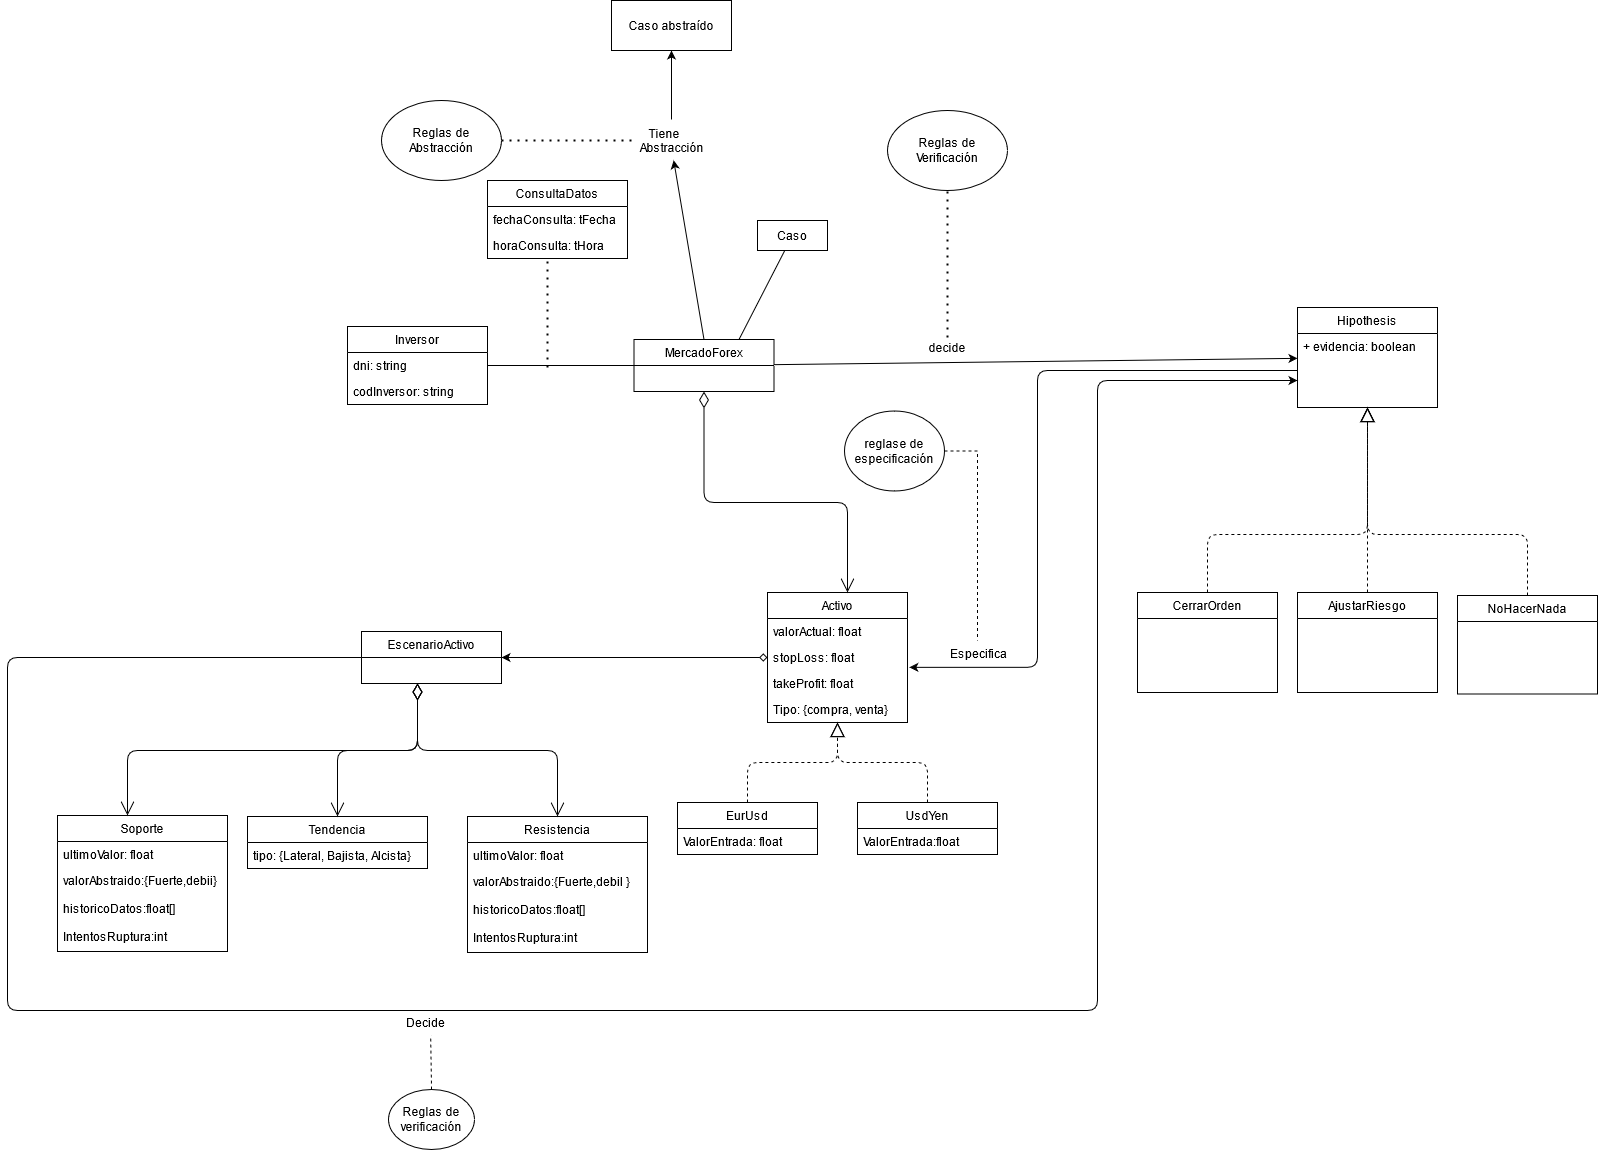
\includegraphics[scale=0.25]{imagenes/DiagramaCompleto.png}
  \caption{\label{fig:DominioCompleto}Esquema completo del dominio}
\end{figure}
\newpage

\section{Fase de refinamiento}
\subsection{Validación de modelo}

Una vez definidos ya todos los elementos anteriores, procedemos a ver cómo se irían desarrollando los ejemplos expuestos anteriormente.

\subsubsection{Escenario 1}
El inversor ya tiene abierta una operativa de compra en el mercado de Forex, donde según el precio del mercado actualmente esta indicando que el precio ha ido a favor del inversor y como esta operativa esta gestionada por un sistema y ese tiene que tomar deciciones en función de como se comporta el mercado. En las Tablas \ref{tab:EjemploEscenario11} y \ref{tab:EjemploEscenario12} muestra un desglose:

\begin{table}[H]
  \centering
  \resizebox{18,0cm}{!}{
    \begin{tabular}{|c|c|c|}
      \hline
      \multicolumn{1}{|c}{\textbf{Dominio}} & \multicolumn{1}{|c|}{\textbf{Modelo}}& \multicolumn{1}{|c|}{\textbf{Explicación}}\\
      \hline \hline      
      \multicolumn{1}{|p{4.0cm}|}{\centering Recibe información que el precio del EURUSD comprado en una situación anterior esta a favor del inversor además de romper una resistencia fuerte}& \multicolumn{1}{|p{10.0cm}|}{\centering \textbf{Caso:}ValorActual = 1.19665 y resistencia = 1.19200 } & \multicolumn{1}{|p{4.0cm}|}{\centering LLega una peticion con los datos del caso.}\\
      \hline
      \multicolumn{1}{|p{4.0cm}|}{\centering Datos obtenidos del caso}& \multicolumn{1}{|p{10.0cm}|}{\centering \textbf{Abstraído:}\\MercadoForex.Activo.EscenarioActivo.\\Resistencia.ultimoValor > (max(MercadoForex.Activo.EscenarioActivo.Resistencia.\\historicoDatos) y MercadoForex.Activo.\\EscenarioActivo.Resistencia.intentosRuptura > 3) entonces EscenarioActivo.Resistencia.valorAbstraido = Fuerte } & \multicolumn{1}{|p{4.0cm}|}{\centering Se abstrae la información acerca del tipo de resistencia a partir de los datos obtenidos}\\
      \hline     
      \multicolumn{1}{|p{4.0cm}|}{\centering se recibe la información de la resistencia y del valor del activo}& \multicolumn{1}{|p{10.0cm}|}{\centering \textbf{Cover:}\\Tenemos MercadoForex.Activo.valorActual > EscenarioActivo.Resistencia.ultimoValor y EscenarioActivo.Resistencia.valorAbstraido = Fuerte entonces Hypothesis = (CerrarOrden,NoHacerNada,AjustarRiesgo) } & \multicolumn{1}{|p{4.0cm}|}{\centering A partir de los datos de la resistencia superada se selecionan las hipotesis posibles}\\
      \hline     
    \end{tabular}
  }
	\caption{\label{tab:EjemploEscenario11}Desglose del funcionamiento del sistema para el escenario 1}
\end{table}

\begin{table}[H]
  \centering
  \resizebox{18,0cm}{!}{
    \begin{tabular}{|c|c|c|}
      \hline
      \multicolumn{1}{|c}{\textbf{Dominio}} & \multicolumn{1}{|c|}{\textbf{Modelo}}& \multicolumn{1}{|c|}{\textbf{Explicación}}\\
      \hline \hline      
      \multicolumn{1}{|p{4.0cm}|}{\centering Se reciben las hipotesis posibles}& \multicolumn{1}{|p{10.0cm}|}{\centering \textbf{Select:}\\Se selecciona aleatoriamente AjustarRiesgo\\} & \multicolumn{1}{|p{4.0cm}|}{\centering De las hipotesis se selecciona una a evaluar de forma aleatoria}\\
      \hline  
      \multicolumn{1}{|p{4.0cm}|}{\centering Se recibe la hipotesis seleccionada}& \multicolumn{1}{|p{10.0cm}|}{\centering \textbf{Specify:}\\Se espera que la tendencia sea alcista \\} & \multicolumn{1}{|p{4.0cm}|}{\centering Se especifica el valor de una situacion, necesaria para que la hipotesis pueda llegar a ser valida}\\
      \hline
      \multicolumn{1}{|p{4.0cm}|}{\centering Se reciben los datos del escenario activo}& \multicolumn{1}{|p{10.0cm}|}{\centering \textbf{Obtain:}\\Tenemos: Mercado.Forex.Activo.EscenarioActivo.Tendencia = {Alcista}} & \multicolumn{1}{|p{4.0cm}|}{\centering Se obtiene el valor de la tendencia}\\
      \hline
      \multicolumn{1}{|p{4.0cm}|}{\centering Se reciben las hipotesis y la tendencia}& \multicolumn{1}{|p{10.0cm}|}{\centering \textbf{Verify:}\\Tenemos: Mercado.Forex.Activo.EscenarioActivo.Tendencia = {Alcista} y Hiphotesis=\{AjustarRiesgo,NoHacerNada,CerrarOrden\} entonces AjustarRiesgo.evidencia = True, NoHacerNada.evidencia = False, CerrarOrden.evidencia = False} & \multicolumn{1}{|p{4.0cm}|}{\centering Se contrastan las evidencias encontradas con todas las hipotesis}\\
      \hline
    \end{tabular}
  }
	\caption{\label{tab:EjemploEscenario12}Desglose del funcionamiento del sistema para el escenario 1}
\end{table}



